\documentclass[11pt]{article}

\usepackage{comment} % enables the use of multi-line comments (\ifx \fi) 
\usepackage[a4paper,margin=1cm]{geometry}
\usepackage[utf8]{inputenc}
\usepackage[ngerman]{isodate}
\usepackage{gensymb}
\usepackage[x11names]{xcolor}
\usepackage{graphicx}
\usepackage{booktabs}% http://ctan.org/pkg/booktabs
\usepackage{makecell}
\usepackage{tabularx}
\usepackage{amsmath}
\usepackage{amssymb}
\usepackage{array}
\usepackage{wrapfig}
\usepackage{subcaption}
\usepackage{csquotes}
\usepackage{lscape}
\usepackage{afterpage}
\usepackage{listingsutf8}
\usepackage{geometry}
\usepackage{chngcntr}
\usepackage{multicol}
\usepackage{xcolor}
\usepackage{pifont}
\usepackage{outlines}
\usepackage{breqn}
\usepackage{textcomp}
\usepackage{bm}
\usepackage{enumitem}
\usepackage{hyperref}
\usepackage{mdframed}
\usepackage{scalerel}
\usepackage{stackengine}
\usepackage{mathtools}
\usepackage{qtree}
% Strikethrough text
\usepackage[normalem]{ulem}

% Code highlighting
\usepackage{minted}
\surroundwithmdframed{minted}

% Be able to caption equations and float them in place
\usepackage{float}
\usepackage{caption}

\newmdtheoremenv{theorem}{Theorem}

\DeclareCaptionType{equ}[Equation][List of Equations]

\counterwithin{figure}{section}

\AtBeginDocument{\counterwithin{lstlisting}{section}}

\geometry{a4paper, margin=1in}

\renewcommand*{\thead}[1]{\bfseries #1}
\newcommand{\code}[1]{\texttt{#1}}
\def\doubleunderline#1{\underline{\underline{#1}}}

\newcommand\equalhat{\mathrel{\stackon[1.5pt]{=}{\stretchto{%
				\scalerel*[\widthof{=}]{\wedge}{\rule{1ex}{3ex}}}{0.5ex}}}}

\newcommand\defeq{\mathrel{\overset{\makebox[0pt]{\mbox{\normalfont\tiny def}}}{=}}}

\newcolumntype{C}{>{\centering\arraybackslash}X}

\DeclarePairedDelimiter\abs{\lvert}{\rvert}
\DeclarePairedDelimiter\norm{\lVert}{\rVert}


\definecolor{lightgray}{rgb}{.9,.9,.9}
\definecolor{darkgray}{rgb}{.4,.4,.4}
\definecolor{purple}{rgb}{0.65, 0.12, 0.82}
\definecolor{darkgreen}{rgb}{0.05,0.56,0.06}
\definecolor{mauve}{rgb}{0.8863,0.5216,1}

\setcounter{tocdepth}{3}
\setcounter{secnumdepth}{3}

\graphicspath{{./img/}}

\begin{document}

\title{Optimisation HS19}
\author{Pascal Baumann\\pascal.baumann@stud.hslu.ch}
\maketitle

For errors or improvement raise an issue or make a pull request on the \href{https://github.com/KilnOfTheSecondFlame/mse_summaries}{github repository}.

\tableofcontents

\newpage

\section{Introduction}
The field of Optimisation can be separated into two distinct fields:
\begin{itemize}
	\item Quantitative Analysis and Optimisation:\\
	Based on quantifiable information and knowledge, such as numerical, measurable data, mathematical models and algorithms
	\item Qualitative Analysis and Optimisation:\\
	Based on non-quantifiable information and knowledge, such as informal facts, verbal description of processes and procedures, unstructured information, experience, and implicit knowledge
\end{itemize}
In this summary only the former will be discussed, although the latter is often encountered in a business consulting setting (often up to 80\%).

We differentiate further between \emph{Continuous Optimisation}, where there are infinitely many solutions represented by continuous variables, and \emph{Discrete Optimisation}, with only finitely many solutions represented by integer variables. The main body of theory for continuos optimisation is \emph{Local Optimisation}, whose methodology is usually based on first and second order derivatives. For discrete optimisation there exists a trivial, finite solution algorithm, the Enumeration of all solutions, though this is often impracticable for practical purposes, where the goal is to find good, or preferably optimal, solutions within reasonable time.

\subsection{Linearity}

Because discrete optimisation is concerned with a finite amount of solutions, which can be represented by a list of variables. This list is a finite set in n-dimensional space, whose contour is linear (due to the finiteness of the set). The convex hull of a finite set of points is a convex polyhedron, and every discrete optimisation problem can be modelled as a linear problem.

\begin{figure}[htb]
	\centering
	\includegraphics[width=0.5\linewidth]{img/convex_hull}
	\caption[A convex hull]{}
	\label{fig:convexhull}
\end{figure}

\subsection{Decision Problems}
Discrete Optimisation can help \textbf{decision makers} with support through (i) quantitative models and (ii) qualitative approaches. It's possible that there are multiple \textbf{alternatives} with associated \textbf{consequences}, which may be of a \textbf{deterministic} or \textbf{stochastic} nature. The focus of this course lies in the \textbf{evaluation} of these alternatives with regard to their consequences.

The evaluation of consequences is done on two levels: Satisfaction and Optimisation. Satisfaction means that the consequence has to fulfil certain \textbf{constraints} in order to have a \textbf{feasible} alternative. While Optimisation means that the consequence has to reach the best possible value, that is it must be \textbf{optimal} among all feasible alternatives.

\section{Mathematical Models}
\subsection{Descriptive Models}
Are also called Evaluation Models and answer the question "What If?" by calculating the resulting consequences of a given alternative.

\begin{figure}
	\centering
	\includegraphics[width=0.8\linewidth,keepaspectratio]{img/descriptive_models}
	\caption{A descriptive model}
	\label{fig:descriptivemodels}
\end{figure}

\subsubsection{Vehicle Dispatching in a Car Rental Company}
\begin{minipage}{0.3\linewidth}
	\centering
	\includegraphics[width=\linewidth,keepaspectratio]{vehicle_dispatch}
\end{minipage}
\begin{minipage}{0.7\linewidth}
	\emph{Consequences}:
	
	\begin{tabularx}{\linewidth}{cX}
		$k_0$ & Total distance of all transfers [km]\\
		$k_i^{Out}$ & Number of vehicles transferred out of location $i$, $i\in I$\\
		$k_j^{In}$ & Number of vehicles transferred into location $j$, $j\in J$
	\end{tabularx}
	\vspace{1em}
	
	\noindent
	\emph{Model}:
	\begin{align*}
		k_0 &= \sum_{i\in I}\sum_{j\in J} c_{ij}\cdot x_{ij}\\
		k_i^{Out} &= \sum_{j\in J}x_{ij}\qquad i\in I \\
		k_j^{In} &= \sum_{i\in I}x_{ij}\qquad j\in J
	\end{align*}
\end{minipage}

\subsection{Optimisation Models}
Are also called Prescriptive Models and answer the question "What's best" through calculating an \textbf{optimal} alternative in the set of all \textbf{feasible} alternatives. This set of feasible solutions is called the \textbf{solution space}, which is defined by \textbf{constraints} and is expressed in form of inequalities and equations. The one selected consequence to be optimised is called the \textbf{objective function}.

\begin{figure}[htb]
	\centering
	\includegraphics[width=0.6\linewidth, keepaspectratio]{img/model_functionality}
	\caption{}
	\label{fig:modelfunctionality}
\end{figure}

With these models the user does not have to specify alternatives, as they are specified by the constraints defining the solution space. The model itself does not calculate the solution however, \textbf{Optimisation algorithms} are needed for this.

\subsubsection{Formulation of an Optimisation Model}
\emph{Sets}:
\begin{itemize}
	\item[$I$] Set of locations, $I={1,2,\dots,n}$
\end{itemize}
\noindent
\emph{Parameters}:
\begin{itemize}
	\item[$a_i$] Number of available vehicles at location $i$, $i\in I$
	\item[$b_j$] Number of requested vehicles at location $j$, $j\in J$
	\item[$c_{ij}$] Distance [km] from location $i$ to location $j$, $i\in I, j\in J$
\end{itemize}
\noindent
\emph{Variables}:
\begin{itemize}
	\item[$x_{ij}$] Number of available vehicles at location $i$, $i\in I$
\end{itemize}
\noindent
\emph{Constraints}:
\begin{align*}
	\sum_{j\in J} x_{ij} &\leq a_i \qquad i\in I\\
	\sum_{i\in I} x_{ij} &\geq b_i \qquad j\in J\\
	x_{ij}&\geq 0 \qquad i\in I,  j\in J
\end{align*}
\noindent
\emph{Objective Function}:
\begin{equation*}
	\min\sum_{i\in I}\sum_{j\in J}c_{ij}x_{ij}
\end{equation*}

\noindent
Optimisation models involve \textbf{mathematical definition of solution space}, and have the information for the construction of feasible alternatives integrated. However, they do not have mechanisms for finding optimal solutions, these require the use of optimisation algorithms. Depending on the model type there are various different algorithms. The field studying optimisation models and algorithms is called \textbf{Operations Research}.

\subsubsection{Notational Conventions}
\begin{itemize}[label=,leftmargin=*, labelindent=2cm, labelsep=1cm]
	\item[$\mathbb{R}, \mathbb{Q}, \mathbb{Z}$] set of real, rational and integer numbers
	\item[$\mathbb{R}_0, \mathbb{Q}_0, \mathbb{Z}_0$] corresponding sets constrained to nonnegative numbers
	\item[$\mathbb{R}^n$] set of $n$-dimensional vectors with components in $\mathbb{R}$
	\item vectors are regarded as \textbf{column} vectors
	\item[$S^n$] set of $n$-dimensional vectors with components in $S$\\
	$\{0,1\}^3$ is the set of binary vectors with length 3
	\item \textbf{vectors} are written in bold face, component in normal face with subscripts
	\item \textbf{multiple vectors} are written using superscripts\\
	$\textbf{x}^1,\textbf{x}^2,\dots,\textbf{x}^i = \begin{pmatrix}
		x_1^i\\
		x_2^i\\
		\vdots\\
	\end{pmatrix}$
	\item[$\mathbb{R}^{{m\times n}}$] set of $m\times n$-dimensional matrices ($m$ rows, $n$ columns) with elements in $\mathbb{R}$
	\item[$S^{m\times n}$] set of $m\times n$-dimensional matrices with elements in $S$
	\item \textbf{Matrices} are written in bold face and capitalised, elements in normal face with subscripts
	\item Special notation:\\
	\emph{$i$-th row} of matrix $\textbf{A}$ is denoted $\textbf{a}^{i}$\\
	\emph{$j$-th column} of matrix $\textbf{A}$ is denoted $\textbf{A}_j$
	\item[$S' \subseteq S$] $S'$ is a subset or equal to set $S$
\end{itemize}

\subsubsection{Problem Formulation}
\begin{minipage}{\textwidth}
	\renewcommand{\arraystretch}{1.5}
	\begin{tabularx}{\linewidth}{l X}
		\textbf{General Optimisation Problem}: & $\prod: \max\{f(\textbf{x}):\textbf{x}\in S\}$\\
		Decision variables: & $\textbf{x} = (x_1,x_2,\dots,x_n)^{\text{T}}\in\mathbb{R}^n$\\
		(Feasible) solution: & $\textbf{x} \in S$\\
		Solution space: & $s\subseteq\mathbb{R}^n$\\
		Objective function: & $f: S\rightarrow\mathbb{R}$\\
		\textbf{Optimal solution}: & $\textbf{x}^* \in S$ such that $f(\textbf{x}^*)\geq f(\textbf{x}) \forall \textbf{x} \in S$\\
		\textbf{Optimum}: & $f(\textbf{x}^*)$
	\end{tabularx}
\end{minipage}

\subsubsection{Conditions for Existence of Optimum}
\begin{minipage}{\textwidth}
	\renewcommand{\arraystretch}{1.5}
	\begin{tabularx}{\linewidth}{l X}
		\textbf{Feasibility}: & $S\neq\emptyset$\\
		\textbf{Boundedness}: & feasible, $\exists\omega:f(\textbf{x})\leq\omega\forall \textbf{x}\in S$\\
		\textbf{Closedness}: & feasible, bounded, optimum exists
	\end{tabularx}
\end{minipage}
\paragraph{Example for Infeasibility} $\max\{x_1: 2x_1 + 4x_2 = 5, \textbf{x}\in\mathbb{Z}^2\}$
\paragraph{Example for Unboundedness} $\max\{x_1: 2x_1 + 4x_2 = 5, \textbf{x}\in\mathbb{R}^2\}$
\paragraph{Example for Unclosedness} $\max\{x_1: x_1 \leq 1, \textbf{x}\in\mathbb{R}\}$

\subsubsection{Definition of Solution Space}
\begin{enumerate}[label=\roman*)]
	\item \textbf{Functional Constraints}:\\
	$S = \{ \textbf{x}\in G_1\times\dots\times G_n : g_i(\textbf{x})\leq 0, h_j (\textbf{x}) = 0, i=1,\dots,p,j=1,\dots,q \}$ where $G_i = \mathbb{R},\mathbb{Z},\{0,1\},\dots$
	\item \textbf{Non-Functional Constraints}:\\
	$S = \{ \textbf{x}\in G_1\times\dots\times G_n : "\textbf{x} \text{ has certain properties}" \} $
\end{enumerate}

\paragraph{Maximisation and Minimisation} $\max\{f(\textbf{x}):\textbf{x}\in S\} = - \min\{-f(\textbf{x}):\textbf{x}\in S\}$

\subsection{Definitions and Concepts}

\subsubsection{Problems and Problem Instances}
\textbf{Problem}:
\begin{equation*}
	\max\{\sum_{j=1}^{n}c_j x_j:\sum_{j=1}^{n}a_j x_j \leq b, \textbf{x}\in \mathbb{R}^n\}
\end{equation*}
\noindent
\textbf{Instance}: Defining numerical parameters $n,\textbf{a},b,\textbf{c}$
\begin{equation*}
\max\{4x_1 + 7 x_2 : 3x_1 + 5 x_2 \leq 17, \textbf{x}\in \mathbb{R}^2\}
\end{equation*}

\subsubsection{Neighbourhoods and Local Optima}
To define the concept of a local optimum a notion of a local neighbourhood is needed. The idea: A solution $\textbf{x}\in S$ is locally optimal, if it is the best solution within a certain neighbourhood $N(\textbf{x})$. A neighbourhood is a set of neighbour solutions: $N(\textbf{x})\subseteq S (\textbf{x} \in N(\textbf{x})\text{ is assumed})$. In general the Euclidean (or $\varepsilon$-) neighbourhood is used: open sphere around $\textbf{x}$ with radius $\varepsilon$. However, often other neighbourhoods are used in \textbf{discrete optimisation}.

\paragraph{General Neighbourhood: A Set-Valued Function} Neighbourhood $N: S \rightarrow P(S)$ where $S\subseteq \mathbb{R}^n$, $P(S)$ Powerset of $S$, $\textbf{x} \mapsto N(\textbf{x})$ (Powerset $P(S)$ of a set $S$ is the set containing all subsets of $S$)

Neigbour Solutions: $N(\textbf{x}) \subseteq S$\quad where $x\in N(\textbf{x})$ assumed

\paragraph{Euclidean Neighbourhood, $\varepsilon$-Neighbourhood} $N_\varepsilon (\textbf{x})=\{\textbf{y}\in\mathbb{R}^n:\norm{\textbf{y}-\textbf{x}}<\varepsilon\} \quad \text{where }\varepsilon>0$, Euclidean Norm: $\norm{\textbf{x}} = \sqrt{\textbf{x}^2} = \sqrt{x_1^2+\dots+x_n^2}$. It's a fundamental neighbourhood concept in analysis, and describes the geometric or topological proximity between points. Local optimality (with respect to $N_\varepsilon$) therefore refers to $\textbf{x}$ being the best solution in the neighbourhood $N_\varepsilon(\textbf{x})$.

\begin{figure}[tbh]
	\centering
	\includegraphics[width=0.6\linewidth,keepaspectratio]{euclidean_neighbourhood}
	\caption{Visualisation of the Euclidean Neighbourhood}
	\label{fig:euclideanneighbourhood}
\end{figure}

\subsubsection{Local Search Metaheuristics}
The principle of Local Search Methods:
\begin{enumerate}[label=\roman*.]
	\item Given:\\
	A feasible solution: $\textbf{x} \in S$\\
	A neighbourhood function: $\textbf{x} \mapsto N(\textbf{x})$
	\item Repeat:
	\begin{enumerate}
		\item Search for a better solution $\textbf{x}'$ in the neighbourhood $N(\textbf{x})$
		\item If no better solution is found: Stop $\rightarrow$ The current solution $\textbf{x}$ is locally optimal with respect to $N$.
		\item Otherwise: Take $\textbf{x}'$ as the new current solution, $\textbf{x} := \textbf{x}'$
	\end{enumerate}
\end{enumerate}

This search process repeatedly moves from current solution $\textbf{x}$ to a better neighbourhood solution $\textbf{x}' \in N(\textbf{x})$, until local optimum is reached, this forms a trajectory in solution space.

\subsubsection{Global and Local Optima}
\textbf{Globally optimal solution} $\textbf{x}^*$: $f(x^*)\geq f(\textbf{x})\forall \textbf{x}\in S$\\
\textbf{Locally optimal solution} $\textbf{x}^*$: $f(x^*)\geq f(\textbf{x})\forall \textbf{x}\in N(\textbf{x}) \cap S$\\
The intersection of neighbourhood with $S$ means, that only neighbours that are solutions are considered. Local optimality is always with respect to some neighbourhood $N_\varepsilon(\textbf{x})$.

\subsubsection{Topological Notions}

\begin{figure}[H]
	\centering
	\includegraphics[width=0.8\linewidth, keepaspectratio]{boundary_interior_point}
	\caption{Illustration of interior and boundary point}
	\label{fig:boundaryinteriorpoint}
\end{figure}

\begin{tabularx}{\linewidth}{l X}
	$S$ closed & all boundary points of $S$ are in $S$\\
	$S$ open & all points of $S$ are interior points\\
	$S$ bounded & $S\subseteq \left\{ \textbf{x}\in\mathbb{R}^n:\textbf{a}\leq\textbf{x}\leq\textbf{b} \right\}$\\
\end{tabularx}

\begin{figure}[H]
	\centering
	\includegraphics[width=0.8\linewidth, keepaspectratio]{open_closed_sets}
	\caption{Illustrated difference between open and closed sets}
	\label{fig:openclosedsets}
\end{figure}

\begin{theorem}
	\textbf{Extreme Value Theorem of Weierstrass} Let $S \subseteq \mathbb{R}^n$ be a non-empty, closed, bounded set and $f:S \rightarrow \mathbb{R}$ be continuous. Then $\max\left\{ f(\textbf{x}):\textbf{x}\in S \right\}$ has a finite optimum.
\end{theorem}

This is a fundamental theorem in Analysis and Continuous Optimisation.

\paragraph{Level Sets} Given the graph of a function $f:S\mapsto \mathbb{R}: H = \left\{ (\textbf{x},f(\textbf{x})):\textbf{x}\in S \right\}$, a level set for level $\alpha$ is $L_\alpha = \left\{ \textbf{x}\in S:f(\textbf{x}) = \alpha \right\}$. When the number of variables is two, a level set is generally a curve and called a level curve or contour line.

\begin{figure}[H]
	\centering
	\includegraphics[width=0.6\linewidth, keepaspectratio]{level_set_method}
	\caption{Illustration of level sets}
	\label{fig:levelsetmethod}
\end{figure}

\subsection{Convex Optimisation}
Convex optimisation of two points $\textbf{x}^1, \textbf{x}^2\in\mathbb{R}^n$:
\begin{align*}
	\textbf{x} &= \lambda\textbf{x}^1 + (1-\lambda) \textbf{x}^2\qquad\text{for some }\lambda\in\mathbb{R}\text{ with }0\leq\lambda\leq 1\\
	\textbf{x} &= \textbf{x}^2 + \lambda(\textbf{x}^1 - \textbf{x}^2)\qquad\text{for some }\lambda\in\mathbb{R}\text{ with }0\leq\lambda\leq 1
\end{align*}

\noindent
Geometrically this can be understood as a convex combination of $\textbf{x}^1$ and $\textbf{x}^2$ that lies on the line between $\textbf{x}^1$ and $\textbf{x}^2$.

\begin{figure}[H]
	\centering
	\includegraphics[width=0.7\linewidth, keepaspectratio]{convex_combination}
	\label{fig:convexcombination}
\end{figure}

\noindent
A convex combination of multiple points $ \textbf{x}^1, \textbf{x}^2,\dots,\textbf{x}^k\in\mathbb{R}^n$ takes the form:
\begin{equation*}
	\textbf{x} = \sum_{i=1}^{k} \lambda_i \textbf{x}^i\qquad \text{for some }\boldsymbol{\lambda}\in\mathbb{R}^k\text{ with }0\leq\lambda\leq 1\text{ and }\sum_{i=1}^{k} \lambda_i = 1
\end{equation*}
\noindent
Expressed in words: A convex combination is a linear combination with non-negative coefficients that sum up to 1.

\paragraph{Convex set} $S\subseteq\mathbb{R}^n$:
\begin{equation*}
	\lambda\textbf{x}^1 + (1-\lambda)\textbf{x}^2 \in S \quad\forall\textbf{x}^1,\textbf{x}^2\in S\text{ and all }\lambda\in\mathbb{R}, 0\leq\lambda\leq 1
\end{equation*}
\noindent
Expressed in words: A set $S$ is convex if the line between two arbitrary points of $S$ is entirely contained in $S$.
\begin{figure}[H]
	\centering
	\includegraphics[width=0.8\linewidth, keepaspectratio]{convex_set}
	\caption{Illustration of convex and non-convex sets}
	\label{fig:convexset}
\end{figure}

\paragraph{Convex function} $f:S\rightarrow\mathbb{R}$, where $S$ convex:
\begin{equation*}
	f(\lambda\textbf{x}^1 + (1-\lambda)\textbf{x}^2) \leq \lambda f(\textbf{x}^1) + (1-\lambda)f(\textbf{x}^2)\qquad 0\leq\lambda\leq 1, \textbf{x}^1,\textbf{x}^2 \in S
\end{equation*}

\paragraph{Concave function} $f:S\rightarrow\mathbb{R}$, where $S$ convex:
\begin{equation*}
f(\lambda\textbf{x}^1 + (1-\lambda)\textbf{x}^2) \geq \lambda f(\textbf{x}^1) + (1-\lambda)f(\textbf{x}^2)\qquad 0\leq\lambda\leq 1, \textbf{x}^1,\textbf{x}^2 \in S
\end{equation*}

\begin{figure}[H]
	\centering
	\includegraphics[width=0.7\linewidth, keepaspectratio]{convex_function}
	\label{fig:convexfunction}
\end{figure}

\noindent
In convex optimisation a linear function can be convex and concave, both $\min\left\{ f(\textbf{x}:\textbf{x}\in S) \right\}$ with $f$ convex and $S$ convex, and $\max\left\{ f(\textbf{x}:\textbf{x}\in S) \right\}$ with $f$ concave and $S$ convex are \textbf{convex optimisation problems}.
\begin{theorem}
	In a convex optimisation problem, local optimums is a global optimum.
\end{theorem}

\begin{figure}[H]
	\centering
	\includegraphics[width=0.7\linewidth, keepaspectratio]{convex_optimisation}
	\label{fig:convexoptimisation}
\end{figure}

\paragraph{Convex programming}: $\max\{ f(\textbf{x}):g_i (\textbf{x})\leq b_i , i\in I, \textbf{x} \in \mathbb{R}^n \}$ where $f$ concave and $g_i$ convex.\\
\textbf{Proposition}: $S = \{ \textbf{x}\in\mathbb{R}^n :g_i (\textbf{x})\leq b_i ,i\in I \}$ is convex (intersection of convex sub-level sets).

\section{Linear Programming}
\subsection{Problem Formulation}
Assumptions and notation:

\begin{itemize}[label=-,noitemsep,nosep]
	\item $\textbf{x}\in\mathbb{R}^n$
	\item $ \textbf{A}\in\mathbb{R}^{m\times n} $
	\item $ \textbf{b}\in\mathbb{R}^m $
	\item $ \textbf{c}\in\mathbb{R}^n $
	\item $ I = \{1,\dots,m\} $
	\item $ J = \{1,\dots,n\} $
	\item $ \textbf{a}^i\in\mathbb{R}^n $ is $i$-th row of $\textbf{A}$
	\item $ \textbf{A}^j\in\mathbb{R}^m $ is $j$-th column of $\textbf{A}$
\end{itemize}

\paragraph{Linear function} $f: \mathbb{R}^n\rightarrow\mathbb{R}$
\begin{equation*}
	f(\textbf{x}) = a_1 x_1+a_2 x_2+\cdots+a_n x_n = \sum_{j=1}^{n} a_j x_j = \textbf{a}^T\textbf{x}\quad(\textbf{a}\in\mathbb{R}^n)
\end{equation*}

\paragraph{Linear inequality} $\sum_{j=1}^{n}a_{ij}x_j\leq b_{i}, i\in I$ or $\textbf{a}^i\textbf{x}\leq b_j, i\in I$ or $\textbf{A}\textbf{x}\leq\textbf{b}$. This is analogous for linear inequalities of type "$\geq$" and linear equations "$=$". The general definition of linear functions $f$ is as follows:
\begin{equation*}
	f(\alpha\textbf{x} + \beta\textbf{y}) = \alpha f(\textbf{x})+\beta f(\textbf{y})\quad (\alpha,\beta\in\mathbb{R})\quad\text{Linearity}
\end{equation*}

\noindent
A linear program (LP) should minimise a linear objective function subject to linear constraints (linear inequalities or linear equalities)


\subsubsection{General Form of a Linear Program}
\begin{itemize}[label=,noitemsep,nosep, leftmargin=0.25cm]
	\item $ \min/\max \textbf{c}^T\textbf{x} $
	\item $ \textbf{a}^i\textbf{x}\leq b_i, i\in I_1 $
	\item $ \textbf{a}^i\textbf{x} = b_i, i\in I_2 $
	\item $ \textbf{a}^i\textbf{x}\geq b_i, i\in I_3 $
	\item $ x_j \geq 0, j\in J_1 $
	\item $ x_j \text{ free}, j\in J_2 $
	\item $ x_j \leq 0, j\in J_3 $
\end{itemize}

\subsubsection{Canonical Form of a Linear Program}
\begin{tabularx}{\linewidth}{p{0.5\linewidth} p{0.5\linewidth}}
	$\max \textbf{c}^T \textbf{x}$ & $\min \textbf{c}^T \textbf{x}$\\
	$ \textbf{a}^i\textbf{x} \leq b_i, i\in I $ & $ \textbf{a}^i\textbf{x} \geq b_i, i\in I $\\
	$ x_j \geq 0, j\in J $ & $ x_j \geq 0, j\in J $
\end{tabularx}

\subsubsection{Standard Form of a Linear Program}
\begin{itemize}[label=,noitemsep,nosep, leftmargin=0.25cm]
	\item $ \min/\max \textbf{c}^T\textbf{x} $
	\item $ \textbf{a}^i\textbf{x} = b_i, i\in I $
	\item $ x_j \geq 0, j\in J $
\end{itemize}

\subsubsection{Inequality Form of a Linear Program}
\begin{tabularx}{\linewidth}{p{0.5\linewidth} p{0.5\linewidth}}
	$\max \textbf{c}^T \textbf{x}$ & $\min \textbf{c}^T \textbf{x}$\\
	$ \textbf{a}^i\textbf{x} \leq b_i, i\in I $ & $ \textbf{a}^i\textbf{x} \geq b_i, i\in I $
\end{tabularx}

\subsubsection{Transformations}
\begin{itemize}[label=-]
	\item \textbf{Inequalities to Inequalities}\\
	$\textbf{a}^i\textbf{x}\leq b_i \quad \leftrightarrow \quad - \textbf{a}^i\textbf{x} \geq -b_i$
	\item \textbf{Equalities to inequalities}\\
	$ \textbf{a}^i\textbf{x} = b_i \quad \rightarrow \quad \textbf{a}^i\textbf{x}\leq b_i, \textbf{a}^i\textbf{x} \geq b_i $
	\item \textbf{Inequalities to equalities}\\
	$ \textbf{a}^i\textbf{x} \leq b_i \quad \rightarrow \quad \textbf{a}^i\textbf{x} + x_i^s = b_i, x_i^s\geq 0$ \qquad slack variable\\
	$ \textbf{a}^i\textbf{x} \geq b_i \quad \rightarrow \quad \textbf{a}^i\textbf{x} - x_i^s = b_i, x_i^s\geq 0$ \qquad surplus variable
	\item \textbf{Non-positive to non-negative variables}\\
	$ x_j \leq 0\quad \rightarrow \quad x_j := -\bar{x}_j, \bar{x}_j \geq 0 $
	\item \textbf{Free to non-negative variables}\\
	$ x_j \text{ free} \quad \rightarrow \quad x_j := x_j^+ - x_j^- \qquad x_j^+, x_j^- \geq 0$ 
\end{itemize}

\subsection{Geometric Aspects}
The system of linear inequalities $\textbf{A}\textbf{x}\leq\textbf{b}$ is called linearly indepent, if it's row-vectors $\textbf{a}^i, i\in I$ are linearly independent.

\noindent
\begin{minipage}{0.7\linewidth}
	\textbf{Definition}: Let $a\in\mathbb{R}^n$ and $n\in\mathbb{R}$. Then, $H=\{\textbf{x}\in\mathbb{R}^n:\textbf{a}^T\textbf{x}\leq b\}$ defines a \textbf{Halfspace} (linear: $b=0$, affine: $b\text{arbitrary}$). While $H'=\{\textbf{x}\in\mathbb{R}^n:\textbf{a}^T\textbf{x}= b\}$ is the \textbf{defining hyperplane} of $H$.
\end{minipage}
\begin{minipage}{0.3\linewidth}
	\centering
	\includegraphics[width=\linewidth]{hyperplane}
\end{minipage}

\noindent
\begin{minipage}{0.3\linewidth}
	\centering
	\includegraphics[width=\linewidth]{normal_vector_hyperplane}
\end{minipage}
\begin{minipage}{0.7\linewidth}
	The vector $\textbf{a}$ is therefore the \textbf{normal vector} of the hyperplane $H'=\{\textbf{x}\in\mathbb{R}^n:\textbf{a}^T\textbf{x}= b\}$.
\end{minipage}

\noindent
\begin{minipage}{0.6\linewidth}
	\textbf{Definition}: A \textbf{polyhedron} $P\in\mathbb{R}^n$ is the intersection of a finite number of halfspaces
	\begin{equation*}
		P=\{ \textbf{x}\in\mathbb{R}^n:\textbf{A}\textbf{x}\leq\textbf{b} \} \qquad \text{with }\textbf{A}\in\mathbb{R}^{m\times n}, \textbf{b}\in\mathbb{R}^m
	\end{equation*}
	\noindent
	The defining hyperplanes of $P$ are:
	\begin{equation*}
		\{ \textbf{x}\in\mathbb{R}^n:\textbf{a}^i\textbf{x}=b_i \}, i=1,\dots,m
	\end{equation*}
\end{minipage}
\begin{minipage}{0.4\linewidth}
	\centering
	\includegraphics[width=\linewidth]{polyhedron_hyperplanes}
	\captionof{figure}{Polyhedron in $\mathbb{R}^2$}
\end{minipage}

\vspace{1em}
\noindent
\textbf{Definition}: A \textbf{polytope} in $\mathbb{R}^n$ is a bounded polyhedron, that is a polyhedron $P=\{ \textbf{x}\in\mathbb{R}^n:\textbf{A}\textbf{x}\leq\textbf{b} \}$ for which there exist $\textbf{l},\textbf{u}\in\mathbb{R}^n$ such that:
\begin{equation*}
	P=\{ \textbf{x}\in\mathbb{R}^n:\textbf{A}\textbf{x}\leq\textbf{b}, \textbf{l}\leq\textbf{x}\leq\textbf{u} \}
\end{equation*}

\begin{figure}[H]
	\centering
	\includegraphics[width=0.8\linewidth, keepaspectratio]{polytope}
\end{figure}

\noindent
A polyhedron is a convex set. A point $\textbf{x}\in\mathbb{R}^n$ is a \textbf{vertex} of a polyhedron $P\in\mathbb{R}^n$ if:
\begin{enumerate}[label=\roman*)]
	\item $\textbf{x}\in P$
	\item $\textbf{x}$ is not a strict convex combination of two distinct points $\textbf{x}^1, \textbf{x}^2 \in P$
\end{enumerate}

\noindent
\textbf{Proposition}: $\textbf{x}\in\mathbb{R}^n$ is a \textbf{vertex} of a polyhedron $P=\{ \textbf{x}\in\mathbb{R}^n:\textbf{A}\textbf{x}\leq\textbf{b}\}$ if and only if (iff):
\begin{enumerate}[label=\roman*)]
	\item $\textbf{x}\in P$
	\item $\textbf{x}$ lies on \textbf{ linearly independent defining hyperplanes of} $P$
\end{enumerate}

\noindent
\textbf{Corollary}: $\textbf{x}\in\mathbb{R}^n$ is a \textbf{vertex} of a polyhedron $P=\{ \textbf{x}\in\mathbb{R}^n:\textbf{A}\textbf{x}\leq\textbf{b}\}$ if and only if (iff):
\begin{enumerate}[label=\roman*)]
	\item $\textbf{x}\in P$
	\item there exists selection $B \subseteq {1,\dots,m}$ of $\abs{B} = n$ linearly independent rows of $\textbf{A}$, such that $\textbf{A}_B\textbf{x} = \textbf{b}_B$, or equivalently $\textbf{x} = \textbf{A}_B^{-1} \textbf{b}_B$
\end{enumerate}

\noindent
\textbf{Definition}: Let $P=\{ \textbf{x}\in\mathbb{R}^n:\textbf{A}\textbf{x}\leq\textbf{b}\}$ with $\textbf{A}\in\mathbb{R}^{m\times n}$
\begin{itemize}[label=]
	\item A selection $B\subseteq\{ 1,..,m \}$ of $\abs{B} = n$ linearly independent rows of $\textbf{A}$ is called a \textbf{basic selection}, and the corresponding matrix $\textbf{A}_B$ is called a basis of $\textbf{A}$. The vector $\textbf{x} = \textbf{A}_B^{-1}\textbf{b}_B$ is called the \textbf{basic solution} associated to basis $\textbf{A}_B$. $B, \textbf{A}_B, \text{ and } \textbf{x} = \textbf{A}_B^{-1}\textbf{b}_B$ are called \textbf{feasible} if $\textbf{x}\in P$.
\end{itemize}

\subsection{Simplex Algorithm}

Given a Linear Program $\prod: \max\{ \textbf{c}^T\textbf{x}:\textbf{x} \in P \}$ with  $P=\{ \textbf{x}\in\mathbb{R}^n:\textbf{A}\textbf{x}\leq\textbf{b}\}, \textbf{A}\in\mathbb{R}^{m\times n}, \text{rank}(\textbf{A})=n$, feasible selection $B$.
\begin{enumerate}[label=\roman*)]
	\item Calculate the inverse $\bar{\textbf{A}}=\textbf{A}_B^{-1}$ and the feasible basic solution $\textbf{v} = \bar{\textbf{A}}\textbf{b}_B$
	\item Calculate the reduced costs $\textbf{u}^T = \textbf{c}^T \bar{\textbf{A}}$
	\item If $\textbf{u}\geq \textbf{0}$ then stop. The vertex $\textbf{v}$ is optimal
	\item Otherwise it is $\textbf{u}\ngeq\textbf{0}$. Choose $j\in B$ with $u_j$. Define direction $\textbf{d}=-\bar{\textbf{A}}_j$
	\item Determine $\textbf{A}\textbf{d}$
	\item If $\textbf{A}\textbf{d}\leq \textbf{0}$ then stop, because the Linear Program is unbounded along the direction $\textbf{d}$
	\item Otherwise $\textbf{A}\textbf{d}\leq n\textbf{0}$ holds true, determine $\lambda^*$:
	\begin{equation*}
		\lambda^* = \min\left\{ \frac{b_i - \textbf{a}_i \textbf{v}}{\textbf{a}^i\textbf{d}} : i\in 1,\dots,m , \textbf{a}^i\textbf{d}>0 \right\}
	\end{equation*}
	\item If a minimum is attained for index $k$ perform a basis change:\\
	$B' = B - {j}\cup{k}$. Set $B:=B'$ and start anew.
\end{enumerate}

An example calculation can be found in section \ref{app:sec:simplexalgorithm} in the appendix.

\section{Integer Linear Programming}
\begin{equation*}
	\max\{\textbf{c}^T \textbf{x} : \textbf{x} \in P \cap \mathbb{Z}^n \}\text{ with }P = \{\textbf{x} \in \mathbb{R}^n : \textbf{A}\textbf{x} \leq \textbf{b}\}
\end{equation*}

\begin{figure}[H]
	\centering
	\includegraphics[width=0.7\linewidth]{img/linear_integer_programming}
	\caption{Feasible integer solutions inside convex hull P}
	\label{fig:linearintegerprogramming}
\end{figure}

\paragraph{{\color{red}Binary} Linear Programming}
\begin{equation*}
	\max\{\textbf{c}^T \textbf{x} : \textbf{x} \in P \cap \{0,1\}^n\}\text{ with }P = \{\textbf{x} \in \mathbb{R}^n : \textbf{A}\textbf{x} \leq \textbf{b}\}
\end{equation*}

\paragraph{{\color{red}Mixed Integer} Linear Programming} 
\begin{equation*}
	\max\{\textbf{c}^T \textbf{x} : \textbf{x} \in P \cap \mathbb{Z}_K^n\}\text{ with }P = \{\textbf{x} \in \mathbb{R}^n : \textbf{A}\textbf{x} \leq \textbf{b}\}
\end{equation*}

where $K\subseteq \{1,\dots,n\}$ and $\mathbb{Z}_K^n=\{ \textbf{x}\in\mathbb{R}^n : x_j \in\mathbb{Z}\text{ for } j\in K \}$.

\begin{center}
	\includegraphics[width=0.7\linewidth]{img/mixed_integer_programming}
\end{center}

Often integer linear programming is used when the linear program includes binary variables, that is yes or no decisions, and it belongs to the computationally hardest class of problems NP-complete, where only exponential algorithms are known.

\begin{figure}[tbh]
	\centering
	\includegraphics[width=0.7\linewidth]{img/ilp_rounding_lp}
	\caption{Explanation on why rounding down from LP solutions does not work in ILP}
	\label{fig:ilproundinglp}
\end{figure}

\subsection{Relaxations}
A relaxation of an optimisation problem can be achieved through
\begin{itemize}
	\item \textbf{enlarging the solution space} $S\rightarrow S'$ with $S\subseteq S'$ by removing constraints\\
	\begin{center}
		\includegraphics[width=0.6\linewidth]{img/enlarging_solution_space}
	\end{center}
	\item \textbf{increasing the objective function} $f(\textbf{x})\rightarrow f'(\textbf{x})$ with $f'(\textbf{x}) \geq f(\textbf{x})$ for $\textbf{x}\in S$\\
	\begin{center}
		\includegraphics[width=0.6\linewidth]{img/increasing_objective_function}
	\end{center}
\end{itemize}

\begin{theorem}
	Given an optimisation problem $\prod: \max\{ f(\textbf{x}):\textbf{x} \in S \}$. $\prod': \max\{ f'(\textbf{x}):\textbf{x} \in S' \}$ is a \textbf{relaxation} of $\prod$ if $S\subseteq S'$ and $f'(\textbf{x})\geq f(\textbf{x})$ for $\textbf{x}\in S$.
\end{theorem}

\subsection{Cutting Plane Method}
\begin{theorem}
	Let $P\subseteq \mathbb{R}^n$ be a polyhedro. An inequality $\boldmath{\alpha}^T \textbf{x} \leq \beta$ ($\boldmath{\alpha} \in \mathbb{R}^n, \beta\in\mathbb{R}$) is a {\color{Blue1}valid inequality} for $P$ if $\boldmath{\alpha}^T \textbf{x} \leq \beta$ is valid for all $\textbf{x} \in P$.
	
	A {\color{Blue1}cutting plane} for a polyhedron $P$ is a valid inequality for $P_{\mathbb{Z}}$
\end{theorem}

\subsubsection{Gomory-Chvatal Cut}
\begin{minipage}{0.4\linewidth}
	\begin{center}
		\includegraphics[width=\linewidth]{img/gomory_chvatal_cut_example}
	\end{center}
\end{minipage}
\begin{minipage}{0.6\linewidth}
	\begin{itemize}
		\item Choose arbitraty split $p, 1 - p$, in this case $p = \frac{3}{4}$
		\item Combine inequalitites: $\frac{3}{4} \cdot (1) + \frac{1}{4}\cdot(2)$
		\item $(-\frac{3}{4}\cdot2 x_1 + \frac{3}{4}\cdot x_2) + (\frac{1}{4}\cdot 2 x_1 + \frac{1}{4}\cdot x_2) \leq \frac{3}{4}\cdot 0 + \frac{1}{4}\cdot 6 \Leftrightarrow -x_1 + x_2 \leq 1\textonehalf$
		\item Round down right side
		\item Resulting new inequality (G-C-Cut): $ -x_1 + x_2 \leq 1$
	\end{itemize}
\end{minipage}

\noindent
\textbf{Matrix Notation}
\begin{itemize}
	\item $ \textbf{A} = \begin{pmatrix}
	-2 & 1\\2 & 1\\0 & -1
	\end{pmatrix}
	\quad
	\textbf{b} = \begin{pmatrix}
	0\\ 6\\ -1
	\end{pmatrix}$
	\item $\textbf{u} = (\frac{3}{4},\frac{1}{4}, 0)\geq \textbf{0}$
	\item $\boldmath{\alpha} := \textbf{u}^T\textbf{A} = {\color{Red1}(-1,1)^T}$
	\item $\beta := \textbf{u}^T\textbf{b} = {\color{Red1}1 \frac{1}{2}}$
	\item G-C-Cut: $ {\color{Red1}\boldmath{\alpha}^T\textbf{x} \leq \lfloor\beta\rfloor}$
\end{itemize}

\subsection{Branch-and-Bound Method}
There are two main approaches to solve an Integer Linear Program or a Mixed Integer Linear Program, which are typically combined, \textbf{Branch-and-Bound} and \textbf{Cutting Planes}. Branch-and-Bound is a general solution method, independent from Integer Linear Program, and the general procedure is as follows:

\noindent
\begin{minipage}{0.6\linewidth}
	\begin{enumerate}[label=\arabic*.]
		\item Split the solution space into smaller subspaces or branches iteratively
		\item For each sub-problem or branch:
		\begin{enumerate}[label*=\roman*]
			\item Calculate an upper bound
			\item Calculate a feasible solution
		\end{enumerate}
		\item Use this information to prune certain sub-problems or branches
	\end{enumerate}
\end{minipage}
\begin{minipage}{0.4\linewidth}
	\centering
	\includegraphics[width=0.9\linewidth,keepaspectratio]{branch_and_bound.png}
\end{minipage}

\subsubsection{Example}
We want to find the highest peak in the area accessible by foot. We send Sherpas to climb the mountains and a helicopter to land on said mountain. If they both arrive at the same height, we know that this is a peak that's climbable, otherwise we select the next mountain.

\begin{minipage}{0.8\linewidth}
	\scriptsize
	\Tree
	[.$\prod_0$\\{$[1]$ 5800, 13000} 
		[.$\prod_1$\\{$[3]$ 5800, 10900}
			[.$\prod_5$\\{$[6]$ 7100, 9500} 
				[.$\prod_7$\\{$[7]$ 8200, 9000} 
					[.$\prod_9$\\{$[8]$ 8848, 8848}\\{\color{red}Stop(Opt)} ]
					[.$\prod_{10}$\\{$[9]$ 8600, 8700}\\{\color{red}Stop(Dom)} ] 
				]
				[.$\prod_8$\\{$[10]$ 7900, 8500}\\{Stop(Dom)} ]
			]
			[.$\prod_6$\\{$[5]$ 6400, 6800}\\{Stop(Dom)} ]
		]
		[.$\prod_2$\\{$[2]$ 6500, 12100}
			[.$\prod_3$\\{$[11]$ 7800, 8800}\\{Stop(Dom)} ]
			[.$\prod_4$\\{$[4]$ 6900, 6900}\\{Stop(Opt)} ]
		]
	]
\end{minipage}
\begin{minipage}{0.2\linewidth}
	\begin{itemize}[label=-,leftmargin=*]
		\item[] [1] 5800
		\item[] [2] 6500
		\item[] [4] 6900
		\item[] [6] 7100
		\item[] [7] 8200
		\item[] [8] 8848
	\end{itemize}
\end{minipage}
\clearpage
\subsection{Branch-and-Bound for Integer Linear Programming}
\begin{itemize}
	\item Calculation of an upper bound through LP Relaxation
	\item Branching
	\begin{itemize}
		\item If LP solution is all integer, stop as the current note is optimal
		\item Else choose some fractional variable and round up or down
	\end{itemize}
\end{itemize}
\begin{center}
	\includegraphics[width=0.8\linewidth]{branch_and_bound_ILP}
\end{center}
\begin{itemize}
	\item Calculation of a feasible solution, that is a lower bound
	\begin{enumerate}[label=\roman*.]
		\item Simplistic: Do nothing and hope that LP solution is integer
		\item In practice: Use various heuristic functions
	\end{enumerate}
\end{itemize}

\subsubsection{Branch-and-Bound Method for Integer Linear Programming}
Given an integer linear program $\prod . \max\{\textbf{c}^T\textbf{x} : \textbf{x} \in P\cap\mathbb{Z}^n\}$ with $P = \{ \textbf{x}\in \mathbb{R}^n : \textbf{A}\textbf{x}\leq\textbf{b} \}$
\begin{enumerate}
	\item {\color{DodgerBlue1}Initialisation}: $\hat{r}:=0, P^0 := P, S^0 := P\cap\mathbb{Z}^n, \prod^0 := \max\{\textbf{c}^T\textbf{x} : \textbf{x} \in S^0\},$\\$R:=\{0\}, z^{LB} := -\infty$
	\item {\color{DodgerBlue1}Termination}: If $R = \emptyset$ then stop
	\item {\color{DodgerBlue1}Node Selection}: Choose a node $r \in R$ and set $R := R - \{r\}$
	\item {\color{DodgerBlue1}Bound Calculation and Heuristic Solution}:
	\begin{enumerate}[label=\roman*.]
		\item Calculate upper bound $z_r^{UB}$ for $\prod^r$ by solving the Linear Program relaxation $\prod_{LP}^r : \max\{\textbf{c}^T\textbf{x} : \textbf{x} \in P^r\}$ : Optimum $z^{LP}$ and the optimal solution $\textbf{x}^{LP}$
		\begin{itemize}
			\item If $\prod_{LP}^r$ infeasible then declare $z_r^{UB} := \infty$ and go to step 6
			\item Otherwise $z_r^{UB} = z^{LP}$
		\end{itemize}
		\item Otherwise $z_r^{LB} := -\infty$
	\end{enumerate}
	\item {\color{DodgerBlue1}Global Improvement}: If $z_r^{LB}>z^{LB}$ then set $z^{LB} := z_r^{LB}$ and $\textbf{x}^{LB} := \textbf{x}_r^{LB}$
	\item {\color{DodgerBlue1}Pruning}: Go to step 2 in case of the appearance of one of the following cases
	\begin{itemize}
		\item $z_r^{UB} = \infty$ (Infeasibility)
		\item $z_r^{LB} = z_r^{UB}$ (Optimality)
		\item $z_r^{UB} \leq z^{LB} $ (Dominance) 
	\end{itemize}
	\item {\color{DodgerBlue1}Branching}: Part the set $S^r$ in $S^{\hat{r}+1}$ and $S^{\hat{r}+2}$. Find $j$ with $x_j^{LP} \notin \mathbb{Z}$. Set: $P^{\hat{r}+1} := \{ \textbf{x}\in P^{\hat{r}} : x_j \leq \lfloor x_j^{LP} \rfloor \}, P^{\hat{r}+2} := \{ \textbf{x}\in P^{\hat{r}} : x_j \geq \lfloor x_j^{LP} \rfloor + 1 \}$\\
	Set $ S^q := P^q \cap \mathbb{Z}^n$ for $q\in R^r := \{ \hat{r} + 1,\hat{r} + 2\} \rightarrow $ Consider $\prod^q : \max\{\textbf{c}^T\textbf{x} : \textbf{x} \in S^q\}, q\in R^r$. Set $R := R \cup R^r, \hat{r} := \hat{r} + 2$.
\end{enumerate}

\subsection{Knapsack Problem}

The Branch-and-Bound method for Integer Linear Programming can be illustrated with the \emph{Knapsack Problem}. A finite number of objects $j \in J$ are given. Every object $j \in J$ has a certain volume $a_j \geq 0$ and a certain benefit $c_j \geq 0$. The task is to fill the knapsack with capacity $b$ by a selection of the given objects such that the total volume of the selected objects doesn't exceed the capacity of the knapsack and at the same time the total benefit becomes maximal.

\vspace{1em}
\noindent
\textbf{Sets}:
\begin{itemize}
	\item[$J$] Set of items, $J=\{1,2,\dots,n\}$
\end{itemize}

\noindent
\textbf{Parameters}:
\begin{itemize}
	\item[$a_j$] Weight of item $j\in J$
	\item[$b$] Capacity of the rucksack
	\item[$c_j$] Value of item $j\in J$
\end{itemize}

\noindent
\textbf{Variables}:
\begin{itemize}
	\item[$x_j$] Binary indicator with value 1 if item $j$ is put into the rucksack, $j \in J$
\end{itemize}

\noindent
\textbf{Objective function and constraints}:
\begin{flalign*}
	\max \sum_{j\in J} c_j x_j&&\\
	\sum_{j\in J} a_j x_j \leq b&&\\
	x_j \in \{0,1\}, j\in J&&
\end{flalign*}

\subsubsection{LP Relaxation}
\begin{enumerate}[label=\roman*.]
	\item For every item  $j\in J$ determine the utility coefficient $\frac{c_j}{a_j}$
	\item Sort all items in a decreasing order with regard to the utility coefficient, such that the new order $J = \{1,\dots,n\}$ becomes
	\begin{equation*}
		\frac{c_1}{a_1}\geq\frac{c_2}{a_2}\geq\dots\geq\frac{c_n}{a_n}
	\end{equation*}
	\item Determine $k = \max\{k' : \sum_{j=1}^{k'}a_j \leq b\}$
	\item The optimal solution is given by
	\begin{equation*}
		x_j^{LP} = \left\{ \begin{matrix}
		1 & \text{for } j = 1,\dots, k\\
		\frac{b-\sum_{j' = 1}^{k} a_{j'}}{a_j} & \text{for } j = k + 1\\
		0 & \text{for } j = k + 2,\dots, n
		\end{matrix} \right.
	\end{equation*}
\end{enumerate}

\subsubsection{Heuristic Search}
	\begin{equation*}
		x_j^{LB} = \left\{ \begin{matrix}
			1 & \text{for } j = 1,\dots, k\\
			0 & \text{for } j = k + 1,\dots, n
		\end{matrix} \right.
\end{equation*}

\subsubsection{Definition of the Sub-Problems}
\begin{itemize}
	\item Sub-problems defined by set $J_r^0,J_r^1\subseteq J$
		\begin{equation*}
			x_j^{LP} = \left\{ \begin{matrix}
				0 & \text{for } j \in J_r^0\\
				1 & \text{for } j \in J_r^1\\
				\text{not fixed} & \text{for } for j\in J_r := J - J_r^0 - J_r^1
			\end{matrix} \right.
	\end{equation*}
	\item Sub-problem ${\prod}^r$ given by
	\begin{equation*}
		{\prod}^r : \max \left\{ \sum_{j\in J_r}c_j x_j : \sum_{j\in J_r}a_j x_j  \leq b - \sum_{j\in J_r^1}a_j x_j  \right\}
	\end{equation*}
\end{itemize}

\paragraph{Strategy for choosing a node:} \textcolor{DodgerBlue1}{Depth-First-Search strategy} - next node to process is the one arising from \emph{rounding up} the fractional variable

\section{Continuous Optimisation}
\subsection{Gradient Descent}
Gradient descent is an algorithm to find a local minimum of an (unconstrained multidimensional) function $f$. The idea behind GD is that the function increases in the direction of the gradient, so by going in the opposite direction the function values decrease until a minimum is reached.

\paragraph{Algorithm}
\begin{itemize}
	\item \emph{Initialisation}: Choose starting point $x^0$
	\item \emph{Iteration step} $x^i \rightarrow x^{i+1}$: Determine local gradient $\nabla f(x^i)$ and move by some amount $\beta$ in opposite direction $-\nabla$ to get a new point $x^{i+1}$\\
	Repeat until gradient value is zero or goes below a target threshold
\end{itemize}

\subsubsection{Step Size}
There are different methods to find the optimal step size $\beta$ to balance speed of convergence and risk of overshooting.

\paragraph{Rule 1: Successive Halving of the Step Size}
\begin{equation*}
	x^{i+1} = x^i - \beta \nabla f(x^i)
\end{equation*}
Set $b := 1$ and check whether

\begin{equation}
	f(x^i - \beta \nabla f(x^i)) < f(x^i)
	\label{eq:gradientdescentstep}
\end{equation}

\noindent
If (\ref{eq:gradientdescentstep}) is not satisfied, set $\beta := \frac{\beta}{2}$ and check again. Iterate until (\ref{eq:gradientdescentstep}) is satisfied.

If (\ref{eq:gradientdescentstep}) is satisfied, repeat doubling $\beta := 2\cdot\beta$ as long as function values $f(x^i - \beta \nabla f(x^i))$ are decreasing.

\paragraph{Rule 2: Successive Halving of the Step Size with Subsequent Parabola Fitting}

Improvement of $\beta$ after applying Rule 1: Approximate $f$ near $x^i$ in direction of $-\nabla f(x^i)$ by a quadratic parabola. Consider choosing $x^{i+1}$ according to the minimum of the parabola.

Compute the parabola $P(t) = a\cdot t^2 + b\cdot t + c$ such that
\begin{align*}
	P(0) &= f(x^i)\\
	P(\beta) &= f\left(x^i - \beta\nabla f(x^i)\right)\\
	P(2\beta) &= f\left(x^i - 2\beta\nabla f(x^i)\right)
\end{align*}

\noindent
$P(t)$ attains its minimum in the interval $[0, 2\beta]$ at $\beta^* = - \frac{b}{2a}$. Choose either $\beta$ or $\beta^*$ as the final value of the step size $\beta$, whichever gives the lower function value for $x^{i+1}$.

\begin{align*}
	a &= \frac{1}{2\beta^2} \left[ f(x^i) - 2 f\left(x^i - \beta\nabla f(x^i)\right) + f\left(x^i - 2\beta\nabla f(x^i)\right)\right]\\
	b &= \frac{1}{2\beta} \left[ -3 f(x^i) + 4 f\left(x^i - \beta\nabla f(x^i)\right) - f\left(x^i - 2\beta\nabla f(x^i)\right) \right] \\
	c &= f(x^i)\\
	\beta^* &= \frac{-b}{2a} = \frac{\beta}{2} \cdot \frac{3 f(x^i) - 4 f\left(x^i - \beta\nabla f(x^i)\right) + f\left(x^i - 2\beta\nabla f(x^i)\right)}{f(x^i) - 2 f\left(x^i - \beta\nabla f(x^i)\right) + f\left(x^i - 2\beta\nabla f(x^i)\right)}
\end{align*}

\subsection{Newton's Method}

Newton's method finds the zero of a function through iterative approximation. The method works through laying the tangent $t$ through point $(x^i, f(x^i)$ which has the slope $f'(x_i)$
\begin{equation*}
	t(x) = f'(x^i)(x-x^i) + f(x^i)
\end{equation*}

\noindent
Finding the zero of the tangent yields
\begin{align*}
	t(x) &= 0\\
	f'(x^i)(x-x^i) + f(x^i) &= 0\\
	x - x^i &= - \frac{f(x^i)}{f'(x^i)}\\
	x &= x^i - \frac{f(x^i)}{f'(x^i)}
\end{align*}

\noindent
Therefore the new iteration point is $x^{i+1} = x^i - \frac{f(x^i)}{f'(x^i)}$.

Newton's method applied to the function $f: \mathbb{R} \rightarrow \mathbb{R}$ approximates the zeros of the function. Applied to the derivative $f'$

\begin{equation*}
	x^{i+1} = x^i - \frac{f'(x^i)}{f''(x^i)}
\end{equation*}
\noindent
approximates the zeros of the derivative, that is the stationary points of the function $f$.

For a multi-dimensional function $f: \mathbb{R}^n \rightarrow \mathbb{R}$ the Newton method is
\begin{align*}
	x^{i+1} &= x^i -(H_f(x^i))^{-1} \nabla f(x^i)\\
	\nabla f(x^i) &= \begin{pmatrix}
		\frac{\partial f(x^i)}{\partial x_1}\\
		\frac{\partial f(x^i)}{\partial x_2}
		\vdots\\
		\frac{\partial f(x^i)}{\partial x_n}
	\end{pmatrix}\\
	H_f(x^i) &= \begin{pmatrix}
	\frac{\partial^2 f(x^i)}{\partial x_1\partial x_1} & \frac{\partial^2 f(x^i)}{\partial x_1\partial x_2} & \dots & \frac{\partial^2 f(x^i)}{\partial x_1\partial x_n}\\
	\frac{\partial^2 f(x^i)}{\partial x_2\partial x_1} & \frac{\partial^2 f(x^i)}{\partial x_2\partial x_2} & \dots & \frac{\partial^2 f(x^i)}{\partial x_2\partial x_n}\\
	\vdots & \vdots & \ddots & \vdots\\
	\frac{\partial^2 f(x^i)}{\partial x_n\partial x_1} & \frac{\partial^2 f(x^i)}{\partial x_n\partial x_2} & \dots & \frac{\partial^2 f(x^i)}{\partial x_n\partial x_n}\\
	\end{pmatrix}
\end{align*}

\subsection{Speed of Convergence}

\paragraph{Linear convergence} There is $c\in(0,1)$ and $i_0 \in \mathbb{N}$ such that $\forall i\geq i_0$ we have
\begin{equation*}
	\norm{x^* - x^{i+1}} \leq c \norm{x^* - x^{i}}
\end{equation*}
\emph{Gradient Descent} achieves linear convergence

\paragraph{Superlinear convergence} There is a sequence $\{c_i\} i\in\mathbb{N}$ with $\lim\limits_{n\rightarrow\infty}c_i = 0$ such that
\begin{equation*}
\norm{x^* - x^{i+1}} \leq c_i \norm{x^* - x^{i}}
\end{equation*}
\emph{Newton's Method} achieves superlinear convergence

\paragraph{Quadratic convergence} There is $c > 0$ and $i_0 \in \mathbb{N}$ such that $\forall i \geq i_0$ we have
\begin{equation*}
\norm{x^* - x^{i+1}} \leq c \norm{x^* - x^{i}}^2
\end{equation*}
\emph{Broyden's Method} achieves quadratic convergence

\subsection{Approximating Partial Derivatives}
Computing the partial derivatives of $f$ exactly may be impossible or computationally too expensive. In these cases working with approximations may be preferably.

\paragraph{Approximation for First Order Partial Derivative}
\begin{equation*}
	\frac{\partial f(x)}{\partial x_i} \approx \frac{1}{2\epsilon}\left(f(x_1,x_2, \dots, x_i + \epsilon, \dots, x_n) - f(x_1,x_2, \dots, x_i - \epsilon, \dots, x_n)\right)
\end{equation*}

\paragraph{Approximation for Second Order Partial Derivatives}
\begin{align*}
	\frac{\partial^2 f(x)}{\partial x_i^2} \approx \frac{1}{\epsilon^2} (&f(x_1,x_2, \dots, x_i + \epsilon, \dots, x_n) - 2f(x_1,\dots, x_n) - f(x_1,x_2, \dots, x_i - \epsilon, \dots, x_n))\\
	\frac{\partial^2 f(x)}{\partial x_i \partial x_j} \approx \frac{1}{4\epsilon^2} (&f(x_1,\dots, x_i + \epsilon, \dots, x_j + \epsilon ,\dots, x_n)\\
	 - &f(x_1,\dots, x_i + \epsilon, \dots, x_j - \epsilon ,\dots, x_n)\\
	 - &f(x_1,\dots, x_i - \epsilon, \dots, x_j + \epsilon ,\dots, x_n)\\
	 + &f(x_1,\dots, x_i - \epsilon, \dots, x_j - \epsilon ,\dots,x_n))
\end{align*}

\subsection{Broyden's Method}
Computing and inverting the Hessian matrix $H_f(x^i)$ exactly in the approximate version of Newton's method
\begin{equation*}
	x^{i+1} = x^i - \left( H_f(x^i) \right)^{-1}\nabla f(x^i)
\end{equation*}
\noindent
is computationally expensive.

The idea in quasi-Newton methods is to approximate the inverse of the Hessian $H_f(x^i)$ by some matrix $(A^i)^{-1}$ that can be computed more efficiently. The matrix $H_f(x^i)$ is the multidimensional derivative of the gradient at the point $x^i$ . Hence it makes sense to require that the approximation $A^i$ satisfies

\begin{equation*}
	A^i(x^i - x^{i-1}) = \nabla f(x^i) - \nabla f(x^{i-1})
\end{equation*}

\noindent
Broyden's method exploits the fact that this requirement is satisfied exactly for

\begin{equation*}
	A^i = A^{i-1} + \frac{\left(\left(\nabla f(x^i) - \nabla f(x^{i-1})\right) - A^{i-1} (x^i - x^{i-1})\right) (x^i - x^{i-1})^T}{\norm{x^i - x^{i-1}}^2}
\end{equation*}

\noindent
Define $g^i$ and $d^i$ in order to abbreviate
\begin{align*}
	A^i &= A^{i-1} + \frac{( (\overbrace{\nabla f(x^i) - \nabla f(x^{i-1})}^{:= g^i} - A^{i-1}) (\overbrace{x^i - x^{i-1}}^{:= d^i}) ) (\overbrace{x^i - x^{i-1}}^{:= d^i})^T}{\norm{\underbrace{x^i - x^{i-1}}_{:= d^i}}^2}\\
	&= A^{i-1} + \frac{(g^i - A^{i-1} d^i) {d^i}^T}{\norm{d^i}^2}
\end{align*}

\noindent
The key insight of Broyden’s method is that we do not need to invert $A^i$ explicitly in each step
\begin{equation*}
	x^{i+1} = x^i - (A^i)^{-1}\nabla f(x^i)
\end{equation*}

\noindent
Instead $(A^i)^{-1}$ can be computed by updating $(A^{i-1})^{-1}$ according to the \textbf{Sherman-Morrison formula}.

\begin{theorem}
	Let $A$ be a regular matrix and $u,v$ two vectors. If $u^T A^{-1} \neq -1$ then $A + vu^T$ is regular as well and the following holds true:
	\begin{equation*}
		\left(A+vu^T\right)^{-1} = A^{-1} - \frac{A^{-1}vu^T A^{-1}}{1 + u^T A^{-1}v}
	\end{equation*}
\end{theorem}

\noindent
Using this formula, $(A^i)^{-1}$ can be computed directly from $(A^{i-1})^{-1}$
\begin{align*}
	A^i = \left({\color{DodgerBlue1} A^{i-1}} + \frac{{\color{DarkOrange1} (g^i - A^{i-1}d^i) } {\color{DarkOrchid4} d^i }^T}{{\color{DarkOrange1} \norm{d^i}^2 }}\right)^{-1} &=  ({\color{DodgerBlue1} A} + {\color{DarkOrange1} v}{\color{DarkOrchid4} u }^T )^{-1}\\
	&\overset{\text{SM}}{=} {\color{DodgerBlue1} A}^{-1} - \frac{{\color{DodgerBlue1} A}^-1 {\color{DarkOrange1} v} {\color{DarkOrchid4} u }^T {\color{DodgerBlue1} A}^{-1}}{1 + {\color{DarkOrchid4} u }^T {\color{DodgerBlue1} A}^-1 {\color{DarkOrange1} v} }\\
	&= (A^{i-1})^{-1} - \frac{\left((A^{i-1})^{-1}g^i-d^i\right)(d^i)^T(A^{i-1})^{-1}}{(d^i)^T(A^{i-1})^{-1}g^i}
\end{align*}

\subsubsection{Algorithm}
\begin{enumerate}
	\item \textbf{Initialisation}: Start with $x^0$. Compute $\nabla f(x^0)$, the inverse of the Hessian Matrix $H_f(x^0)$ and set $(A^0)^{-1} = \left(H_f(x^0)\right)^{-1} $. Use this to compute
	\begin{equation*}
		x^1 = x^0 - (A^0)^{-1}\nabla f(x^0)
	\end{equation*}
	\item \textbf{Iteration step}: To compute $x^{i+1}$ from $x^i$, compute $\nabla f(x^i)$, $g^i = \nabla f(x^i) - \nabla f(x^{i-1})$ and $d^i = x^i - x^{i-1}$, then
	\begin{equation*}
		(A^{i})^{-1} = (A^{i-1})^{-1} - \frac{\left((A^{i-1})^{-1}g^i-d^i\right)(d^i)^T(A^{i-1})^{-1}}{(d^i)^T(A^{i-1})^{-1}g^i}
	\end{equation*}
	and set
	\begin{equation*}
		x^{i+1} = x^i - (A^i)^{-1} \nabla f(x^i)
	\end{equation*}
\end{enumerate}

After the first step, $A^i$ or $H_f(x^i)$ is never dealt with explicitly, only $(A^i)^{-1}$ is maintained and updated. This saves significant computer cost, especially for an $n$-dimensional problem, as inverting $A^i$ or $ H_f(x^i)$ explicitly would take $O(n^3)$, while computing the inverse with Sherman-Morrison updates and multiplying by the gradient $\nabla f(x^i)$ can all be done in $O(n^2)$.

\subsection{Aitken's Acceleration Method}
Aitken's $\Delta^2$ method is not a new method for finding local extrema, but can be used to improve the convergence speed of other existing methods that would converge slowly otherwise.

Let $\{x^i\}_{i\in\mathbb{N}}$ be a scalar sequence that converges linearly towards its limit $x^*$. Construct a new sequence $\{y^i\}_{i\in\mathbb{N}}$ from $\{x^i\}_{i\in\mathbb{N}}$ as follows
\begin{align*}
y^i &= x^i - \frac{(x^i - x^{i-1})^2}{x^i - 2x^{i-1} + x^{i-2}}\\
&= x^i - \frac{(\Delta x^i)^2}{\Delta^2 x^i}
\end{align*}
where $\Delta^2 x^i = \Delta(\Delta x^i) = \Delta(x^i - x^{i-1}) \Delta x^i - \Delta x^{i-1}$. Then $\{x^i\}_{i\in\mathbb{N}, i\geq 2}$ converges quadratically towards the same limit $x^*$.

\section{Graph and Network Optimisation}

\begin{theorem}
	A \textbf{graph} $G=(V,E)$ consists of finite $V$ of vertices and a set $E\subseteq V\times V$ of edges. An edge $e \in E$ is of the form $e = (u,v)$ with $u,v\in V$.
	
	A \textbf{weight function} on $G=(V,E)$ is a function assigning a real number to each edge $e\in E$
\end{theorem}

\begin{theorem}
	The \textbf{adjacency matrix} of a graph $G$ with $\abs{N} = n$ is the $n\times n$-matrix with entries
	\begin{equation*}
		a_{ij} = \left\{\begin{matrix}
		1 & \text{if } (u_i, u_j) \in E\\
		0 & \text{if } (u_i, u_j) \notin E
		\end{matrix}
		\right.
	\end{equation*}
\end{theorem}
For an undirected graph, the adjacency matrix is symmetric. For a weighted graph, the adjacency matrix specifies the edge weights.

The \textbf{adjacency list} representation of a graph consists of a doubly linked list for each vertex, specifying all of its neighbours.

\subsection{Depth-First Search}

\begin{center}
	\includegraphics[width=0.6\linewidth]{search_graph_example}
\end{center}

\begin{enumerate}
	\item Start at $a$ and put it on the stack
	\item If there is an unmarked neighbour, go there and put it on the stack
	\item If there is no unmarked neighbour, backtrack and go to step 2.
\end{enumerate}

\paragraph{Stack:} a, b, d, \sout{c}, f, e, \sout{g}, h

\subsection{Breadth-First Search}

\begin{enumerate}
	\item Start at $a$ and put it in queue
	\item Output first vertex from queue. Mark all neighbours and put them in queue. Do so until queue is empty.
\end{enumerate}
\paragraph{Queue:} a, b, d, e, c, f, h, g

\subsection{Spanning Tree}
Given a graph $G(V,E)$ with positive edge weights find a set of edges that connects all vertices of $G$ with minimum weight.

\subsubsection{Optimistic Approach}
Successively build the cheapest connection available that is not redundant.

\begin{center}
	\includegraphics[width=0.6\linewidth]{spanning_tree_optimistic}
\end{center}

\subsubsection{Pessimistic Approach}
Successively rule out the most expensive line that is not absolutely needed.

\begin{center}
	\includegraphics[width=0.6\linewidth]{spanning_tree_pessimistic}
\end{center}

\subsubsection{Prim's Algorithm}
Choose an arbitrary start vertex $v_0$ and set $M = \{v_0\}$. Iteratively add the cheapest to reach vertex in $V\setminus M$ to the current set $M$. Select the corresponding edge. Continue until $M = V$.

The edges selected in this way form a minimum-weight spanning tree.

\subsubsection{Kruskal's Algorithm}

Set $M= \{\}$. Iteratively add the cheapest edge in $E\setminus M$ that connects two vertices that are not yet connected by edges in $M$. Continue until all vertices are connected by edges in $M$.

The edges in $M$ form a minimum-weight spanning tree. Kruskal's Algorithm is equivalent to the optimistic approach.

Prim's and Kruskal's Algorithms are both greedy algorithms.

\subsection{Shortest Paths}
Given a graph $G(V,E)$, two vertices $u,v\in V$ with positive weights, interpreted as distances.

\textbf{Dijkstra's Algorithm} can be used to find a shortest path in $G$ connecting $u$ to $v$ or a shortest path from a start vertex $v_0$ to \emph{all} other vertices. And the \textbf{Floyd-Warshall Algorithm} can be used as an efficient solution to find the shortest path between \emph{all pairs} of vertices.

\subsubsection{Dijkstra's Algorithm}
\begin{enumerate}
	\item \textbf{Initialisation}: Set $V_0 = \{v_0\}$, $E_0 = \{\}$ and $I(v_0) = 0$
	\item Do the following $n-1$ times:\\
	$V_i = \{v_0, \dots, v_i\}$ and $E_i = \{e_0, \dots, e_i\}$ are the sets of vertices and edges already visited. For each edge ${\color{Blue1} e = (u,v)}$ with ${\color{Blue1} u\in V_i)}$ and ${\color{Blue1} v\in V\setminus V_i}$ compute ${\color{Blue1} l(u) + \text{weight}(e)}$. Choose the edge minimising this as $e_{i+1} = (u_{i+1}, v_{i+1})$.\\
	Set $V_{i+1} = V_i \cup \{v_{i+1}\}, E_{i+1} = E_i \cup \{e_{i+1}\}$ and $l(v_{i+1}) = l(u_{u+1}) + \text{weight}(e_{i+1})$.
\end{enumerate}

\subsubsection{Floy-Warshall Algorithm}

Let $V = \{v_1,\dots,v_n\}$ and let ${\color{Blue1} \text{minPath}(i,j,k)}$ denote the length of a shortest path from $v_i$ to $v_j$ that only uses vertices from $\{v_1, \dots, v_k\}$

\paragraph{Notes}: In the end there should be a ${\color{Blue1}\text{minPath}(i,j,n)}$ for all vertices $v_i$ and $v_j$. ${\color{Blue1}\text{minPath}(i,j,0)}$ is the weight of the edge $(v_i,v_j)$ or $\infty$ if the edge does not exist. Suppose for all $i,j$ the ${\color{Blue1}\text{minPath}(i,j,k)}$ has been computed, then
\begin{equation*}
	{\color{Blue1}\text{minPath}(i,j,k)} = \min\left\{ \begin{matrix}
	{\color{Blue1}\text{minPath}(i,j,k)}\\
	{\color{Blue1}\text{minPath}(i,{\color{Red1}k+1},k)} + {\color{Blue1}\text{minPath}({\color{Red1}k+1},j,k)}
	\end{matrix} \right.
\end{equation*}
The minimum is attained for the second term if it pays off to go via ${\color{Red1}v_{k+1}}$.

Given $G=(V,E)$ with weight function $\omega : E \rightarrow \mathbb{R}$. Find the shortest distances between all pairs of vertices.

\begin{enumerate}
	\item \textbf{Initialisation}:
	\begin{equation*}
		{\color{Blue1}\text{minPath}(i,j,0)} = \left\{ \begin{matrix}
		\omega(v_i,v_j) & \text{if } (v_i,v_j) \in E\\
		\infty & \text{else}
		\end{matrix} \right.
	\end{equation*}
	\item For $k=1,2,\dots,n$ compute:\\
	${\color{Blue1}\text{minPath}(i,j,k)}$ for all $i$ and $j$ according to iteration formula
\end{enumerate}

The values ${\color{Blue1}\text{minPath}(i,j,n)}$ are the shortest distances from $v_i$ to $v_j$.

\begin{center}
	\includegraphics[width=0.7\linewidth]{img/floyd_warshall_algorithm_example}
\end{center}

\subsection{Maximum Network Flow}
An $st$-network $(G,\omega,s,t)$ is a weighted graph $G(V,E)$ with weight function $\omega$ and two distinguished vertices $s,t \in V$, where $s$ is the \textbf{source} and $t$ is the \textbf{target} or \textbf{sink}. What is the maximal flow which can be routed through $G(V,E)$ from $s$ to $t$, respecting the capacity limits given by $\omega$?

\begin{center}
	\includegraphics[width=0.6\linewidth]{img/network_flow_st}
\end{center}

\begin{theorem}
	A graph $G(V,E)$ is \textbf{bipartite} if its vertex set can be split in two parts $A$ and $B$ such that all edges have one vertex in $A$ and one in $B$.
\end{theorem}

\subsection{Ford-Fulkerson Algorithm}
Given $G(V,E)$ with positive capacities $\omega : E \rightarrow \mathbb{R}$, source $s$ and sink $t$, find the maximum flow $F_{s\rightarrow t}$ from $s$ to $t$ through $G$.
\begin{enumerate}
	\item \textbf{Initialisation}: Set the total flow $F_{s\rightarrow t} = $, residual graph $G_R = G$ and edge flows $f(e) = 0\text{ }\forall e\in E$
	\item While there is a path $P$ from $s$ to $t$ in $G_R$
	\begin{itemize}
		\item Determine smallest capacity $g$ along the path $P$
		\item Reduce capacities along $P$ by $g$
		\item Increase capacities of backwards edges by $g$
		\item Delete edges with capacity $0$ in $G_R$
		\item Increase $F_{s\rightarrow t}$ by $g$
		\item Increase flows $f(e)$ along $P$ by $g$
	\end{itemize}
	\item Output $F_{s\rightarrow t}$, $f(e)$, $e\in E$
\end{enumerate}

\begin{center}
	\includegraphics[width=0.8\linewidth]{img/network_flow_ford_fulkerson_01}
\end{center}

\begin{center}
	\includegraphics[width=0.8\linewidth]{img/network_flow_ford_fulkerson_02}
\end{center}

The Ford-Fulkerson algorithm has inefficient behaviour, that if the augmenting paths are chosen arbitrarily, the algorithm might take many iterations to find the maximum flow.

\paragraph{Edmonds-Karp Algorithm} In each iteration, use a \textbf{\emph{shortest}} augmenting path, that is a path from $s$ to $t$ with the fewest number of edges. Can be found with BFS in time $O(\abs{E})$.

\subsection{Max-Flow Min-Cut Theorem}
\begin{theorem}
	An $st$-\textbf{cut} in the graph $G(V,E)$ is a partition of the vertex set into two sets $S$ and $T = V\setminus S$ with $s\in S, t\in T$. The \textbf{value} of such an \emph{st}-cut is the total weight of all edges that go from $S$ to $T$.  The maximum \emph{st} flow equals the minimum value of all possible \emph{st}-cuts.
\end{theorem}

\begin{center}
	\includegraphics[width=0.8\linewidth]{img/max_flow_min_cut}
\end{center}

Often there are several possible maximum flows in a graph, sending different amounts of flow along different edges. The Ford-Fulkerson algorithm can be extended to take into account an additional {\color{Red1}\textbf{cost criterion}}.

Each edge has not only a capacity $\omega$, but also a {\color{Red1}\textbf{cost per flow unit}} going through that edge. The min-cost max-flow algorithm finds a maximum flow with minimum cost.

\begin{center}
	\includegraphics[width=0.4\linewidth]{img/cost_per_flow}
\end{center}

\begin{center}
	\includegraphics[width=0.7\linewidth]{img/cost_per_flow_algorithm}
\end{center}

Until now the Ford-Fulkerson algorithm was used while annotating the costs. Now, look for cycles with negative cost. Send flow along these cycles, respecting the capacities. This does not change the total flow from $s$ to $t$, but decreases the total cost.

\begin{center}
	\includegraphics[width=0.7\linewidth]{img/cost_per_flow_backflow}
\end{center}

\section{Heuristic Optimisation}

A \textbf{heuristic} is a problem-solving strategy that is based on rules of thumb or common sense, possibly also using expert knowledge.

Heuristics are often used when no efficient, exact algorithms are known, or when applying such algorithms would take too long.

This gives the advantage of possibly finding a good solution in a reasonable time, with the drawback that no reliable optimality guarantees can be given.

\begin{center}
	\includegraphics[width=0.6\linewidth]{img/pnp}
\end{center}

Many algorithmic problems are solvable in principle, but no efficient algorithm is known. The classification happens by complexity with regards to growth behaviour with more inputs.

\begin{itemize}[leftmargin=*, labelindent=3cm, labelsep=0.5cm]
	\item[\textbf{P}] Solvable in polynomial time
	\item[\textbf{NP}] Solvable in polynomial time with a non-deterministic machine
	\item[\textbf{NP-hard}] At least as hard as the hardest problems in NP
	\item[\textbf{NP-complete}] In NP and NP-hard
\end{itemize}

A \textbf{metaheuristic} is a general heuristic problem-solving strategy that can be used in optimisation problems. They can be employed both in discrete and continuous problems and both when looking for local and for global optima.

Metaheuristics can sometimes be combined with more rigorous local methods to search for global optima in continuous optimisation problems (hybrid methods).

\subsubsection{Trajectory-based Metaheuristics}
Start with a (random) "solution" and improve it continuously by exploring its neighbourhood and improving the tour.
Thus a trajectory through the solution space is obtained, similar to what is done in Gradient Descent.

Often it is not obvious how to \textbf{define and explore the solution space} or how to \textbf{define a good neighbourhood} for a given problem.

\subsection{Hill Climbing Algorithm}
\begin{enumerate}
	\item \textbf{Initialisation}: Start with random solution. Evaluate initial solution
	\item \textbf{Iteration}: Explore neighbourhood and evaluate new solution candidates. Continue with best solution found, if this improves the target function, otherwise stop as this is a local optimum
	\item Return solution
\end{enumerate}

The implementation of this algorithm is trivial but the size of the neighbourhood or allowed modification steps poses a difficulty. In particular the size of the neighbourhood can be problematic, if chosen too small the algorithm might get stuck quickly without exploring much of the solution space, while a too large size takes a lot of computation time.

As Hill Climbing is a \emph{\textbf{local search}} algorithm it is usually a good idea to have multiple runs with different starting points and take the best solution out of all runs.

\subsubsection{Stochastic Hill Climbing}

\begin{enumerate}
	\item \textbf{Initialization}: Start with random solution. Evaluate initial solution
	\item \textbf{Iteration}: Choose random solution in neighbourhood, that is perform a random modification. Evaluate new solution candidate, and accept it, if it is better. Continue until termination criterion is reached.
	\item Return solution
\end{enumerate}

\noindent
\textbf{Terminate}
\begin{itemize}
	\item if no significant improvement occurs after a fixed number of steps without improvement.
	\item after a fixed total number of iterations or computing time.
	\item when a prescribed target value for the target function is reached.
\end{itemize}

\subsubsection{Continuous Hill Climbing}
Find $\vec{x}$ minimising $f(\vec{x})$ for a given target function $f : \mathbb{R} \rightarrow \mathbb{R}$
\begin{enumerate}
	\item \textbf{Initialisation} $i=0$: Initial solution $x_0$.
	\item \textbf{Iteration} $i \rightarrow i+1$: Sample random solution $y_i$ near $x_i$
	\begin{equation*}
		x_{i+1} = \left\{ \begin{matrix}
		y_i & \text{if } f(y_i) \leq f(x_i)\\
		x_i & \text{if } f(y_i) > f(x_i)
		\end{matrix} \right.
	\end{equation*}
	\item Return solution
\end{enumerate}

This idea is similar to gradient descent, but since this does not rely on derivatives the idea also works in discrete settings.

\subsection{Tabu Search}
The idea behind Tabu search is similar to those in Hill climbing, but the algorithm has a \textbf{memory} and tries to avoid steps that go back to previously evaluated solutions or those that undo the effect of previous steps.

The goal is to \textbf{promote diversity} of the solutions explored, in particular to reduce cyclic behaviour and to escape from local optima.

\begin{enumerate}
	\item \textbf{Initialisation}: Start with random solution. Evaluate initial solution
	\item \textbf{Iteration}: Explore neighbourhood and evaluate new solution candidates. Only consider steps that are not tabu. Proceed with this step, saving the best solution found and updating the tabu list until the termination criterion is reached.
	\item Return solution
\end{enumerate}

The simplest variant of Tabu search is to only store the last solution as a tabu, it would probably be better to keep the last $k$ moves. The goal of the tabus is to help exploring the solution space, that is fostering diversity of the considered solutions.

Further considerations can be made in terms of neighbourhood size, computational requirements, and if evaluations should be approximated or if approximation by updates is possible. Restarting the algorithm should be done in areas not yet explored and exploit the structure of solutions encountered, to learn features ruling out duds or focussing on promising candidates.

It would be beneficial to not flat out disqualify invalid solutions, meaning solutions that violate constraints, but \textbf{penalise} them. \textbf{Strategic oscillation}: Dynamically adjust size of penalty to reach limits of feasiblity. If there are many invalid solutions encountered, the penalty should be increased, if few invalid solutions are encountered, the penalty should be decreased to encourage diversity.

\noindent
\textbf{Variants}
\begin{itemize}
	\item Fixed penalty for invalid solutions
	\item Variable penalty which is adapting to the degree of violation
\end{itemize}

\subsubsection{Stochastic or Randomised Tabu Search}

\begin{enumerate}
	\item \textbf{Initialisation}: Start with random solution. Evaluate initial solution
	\item \textbf{Iteration}: Choose a random solution from the neighbourhood. Evaluate the new solution candidate, if its not in the Tabu list. If a better solution is found, continue with this solution, update the Tabu list and repeat this step. Continue until termination criterion is reached.
	\item Return solution
\end{enumerate}

\subsection{Simulated Annealing}
Similar to hill climbing, but also allow non-improving moves to escape from local optima.

\begin{enumerate}
	\item \textbf{Initialisation}: Start with random solution. Evaluate initial solution
	\item \textbf{Iteration}: Choose a random solution from the neighbourhood and evaluate it. If it is better, accept it. If it is worse, accept it only with some probability. Repeat until termination criterion is reached.
	\item Return solution
\end{enumerate}

\noindent
And with a hard threshold $T$
\begin{enumerate}
	\item \textbf{Initialisation}: Start with $x_0$
	\item \textbf{Iteration}: $x_i \rightarrow x_{i+1}$. Sample random solution $y_i$ in the neighbourhood and accept it to be $x_{i+1}$ with probability $\min\left\{1, e^{\frac{f(x_i) + f(y_i)}{T_i}}\right\}$
\end{enumerate}

\noindent
\begin{itemize}
	\item If $f(y_i) \leq f(x_i) \rightarrow e^{\frac{f(x_i) + f(y_i)}{T_i}} \geq 1$ and $y_i$ is accepted
	\item If $T$ is very large, every solution $y_i$ will be accepted
	\begin{equation*}
		\min\left\{1, e^{\frac{f(x_i) + f(y_i)}{T_i}}\right\} = \min\left\{1, e^{\frac{f(x_i) + f(y_i)}{\infty}}\right\} = \min\left\{1, e^{\pm 0}\right\} = 1
	\end{equation*}
	\item If $T\rightarrow 0$, only solutions better than $y_i$ will be accepted
	\begin{equation*}
	\min\left\{1, e^{\frac{f(x_i) + f(y_i)}{T_i}}\right\} = \min\left\{1, e^{\frac{f(x_i) + f(y_i)}{+0}}\right\} = \min\left\{1, e^{\pm \infty}\right\} = 0\text{ or }1
	\end{equation*}
\end{itemize}

\subsection{Population Based Methods}
The key idea behind the following methods is an evolving \textbf{population} of partial solutions, whose members evolve and adapt individually to the problem and are searching for the optimum. Problem-specific information can be exchanged between the members of the population, and can also be passed on to descendants.

Can be employed both in discrete and continuous problems.

Biological principles serve as an inspiration:
\begin{itemize}
	\item Finite lifespan of individuals and generations
	\item Adaptation by natural selection, survival of the fittest
	\item Inheritance of traits, information is passed on to descendants
	\item Recombination, information is exchanged between parents
	\item Diversification by mutations
	\item Population acquires and cultivates shared knowledge
	\item Local development of populations
\end{itemize}

These principles are the inspiration for evolutionary algorithms, in which populations of solution candidates evolve over time.

\begin{theorem}
	Population-based methods are \textbf{iterative solution techniques} that handle a population of individuals and make them \textbf{evolve according to some rules} that have to be clearly specified. At each iteration, periods of \textbf{self-adaptation} alternate with periods of \textbf{cooperation}.
\end{theorem}

\begin{itemize}
	\item \textbf{Individuals}: Solution candidates or partial solutions
	\item \textbf{Evolutionary process}: constant-size population without survivors from one generation to the next
	\item \textbf{Neighbourhood structure}: Which individuals can exchange information
	\item \textbf{Information sources}: Information gets transmitted between generations
	\item \textbf{Restriction-violating solution candidates}: Discard, repair or penalize?
	\item \textbf{Intensification strategy}: Exploiting neighbourhood by subsequent adjustment of solution candidates
	\item \textbf{Diversification strategy}: Exploring the entire solution space through mutation of the solutions
\end{itemize}

\subsection{Genetic Algorithm}

\subsubsection{Terminology}
A \textbf{generation} is the population at a specific point in time. In each iteration of a genetic algorithm, a new generation is created. The hope is, that over time, the population members of each generation are better and better solutions to the optimisation problem.

The \textbf{genotype} is the encoded form of an individual. While the \textbf{phenotype} is the decoded form of an individual. It does not depend on the choice of encoding. The \textbf{fitness function} is a measure for the quality of a solution candidate in the optimisation problem.

The individual entries in the vector representation of an individual are its \textbf{genes}. They describe the genetic information and the properties of the individuals. The concrete value a gene can take in an individual are called \textbf{alleles}.

The fitness function is the measure for the quality of a solution candidate in the optimisation problem.

\subsubsection{Algorithm}

\begin{enumerate}
	\item \textbf{Initialisation} Random starting population
	\item \textbf{Iteration} Create next generation according to evolutionary principles
	\begin{itemize}
		\item Assign fitness to individuals
		\item Natural selection and choosing predecessors for reproduction
		\item Recombination process
		\item Mutation process
	\end{itemize}
	Repeat until termination criterion is satisfied
	\item Return best individual
\end{enumerate}

\begin{figure}[H]
	\centering
	\includegraphics[width=0.6\linewidth]{img/genetic_algorithm_encoding_problem}
	\caption{The first and most important step is to find a suitable encoding}
	\label{fig:geneticalgorithmencodingproblem}
\end{figure}

\subsubsection{Encoding of an Optimisation Problem}
Desirable would be that a small change in genotype results in a small change in the phenotype. A very simple encoding is often given by a \textbf{standard binary encoding}, however as this has issues with the Hamming distance \textbf{Gray code} is preferable. In continuous optimisation problems \textbf{real-valued encodings} are sometimes more useful.

\vspace{1em}
\noindent
\begin{tabularx}{\linewidth}{|l|X|X|}
	\hline
	decimal & binary & Gray code\\
	\hline
	0 & 000 & 000\\
	1 & 001 (Hamming distance = 1) & 001 (Hamming distance = 1)\\
	2 & 010 (Hamming distance = 2) & 011 (Hamming distance = 1)\\
	3 & 011 (Hamming distance = 1) & 010 (Hamming distance = 1)\\
	4 & 100 (Hamming distance = 3) & 110 (Hamming distance = 1)\\
	5 & 101 (Hamming distance = 1) & 111 (Hamming distance = 1)\\
	6 & 110 (Hamming distance = 2) & 101 (Hamming distance = 1)\\
	7 & 111 (Hamming distance = 1) & 100 (Hamming distance = 1)\\
	\hline
\end{tabularx}

\vspace{1em}
\noindent
Standard Binary $b=b_n\dots b_1 \mapsto$ Gray code $ g= g_n\dots g_1$
\begin{equation*}
	g= b \oplus (b \gg 1)
\end{equation*}

\subsubsection{Replacement Schemes}

\begin{itemize}
	\item \textbf{Generational replacement}: Replace all individuals of a generation
	\item \textbf{Strict elitism}: Keep only $m$ best individuals for next generation
	\item \textbf{Weak elitism}: $m$ best individuals are mutated to obtain the next generation
	\item \textbf{Delete-$n$}: Replace n random individuals 
	\item \textbf{Delete-$n$-last}: Replace $n$ worst individuals and keep the others
	\item \textbf{Retirement home}: Store a part of the population in a "retirement home" for some time, give it another chance to procreate later on in the process
\end{itemize}

\subsubsection{Selection of Predecessors}
\paragraph{Tournament Selection}
\begin{itemize}[label=]
	\item Sample $k$ individuals randomly from the population
	\item Choose best individual with probability $p$
	\item Choose second best individual with probability $(1-p)p$
	\item Choose third best individual with probability $(1-p)^2p$
	\item \quad $\vdots$
	\item Choose $(k-1)$-best individual with probability $(1-p)^{(k-2)}p$
	\item Choose $k$-best individual with probability $(1-p)^{(k-1)}$
\end{itemize}

The larger k, the higher the selection pressure. The advantage of this method is that it is based on ranking and that the selection pressure can be adjusted.

\subsubsection{Recombination}
\begin{minipage}{0.5\linewidth}
	With a \textbf{One-point Crossover} a point is chosen randomly and designated crossover point. The bits are swapped between both parents to generate two offspring. \textbf{Two Point Crossover} follows the same mechanism, but with more crossover points. This method can be generalised for an arbitrary $k$ crossover points. With \textbf{Uniform Crossover} each bit is chosen from either parent with equal probability. Other mixing ratios are sometimes used, resulting in offspring which inherit more genetic information from one parent than the other.
	
	\vspace{3cm}
\end{minipage}
\begin{minipage}{0.5\linewidth}
	\begin{center}
		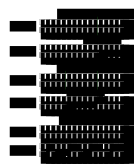
\includegraphics[width=\linewidth,keepaspectratio]{genetic_algorithm_crossovers}
	\end{center}
\end{minipage}

\subsubsection{Recombination for Permutation - PMX Operator}
PMX Crossover is a genetic algorithm operator and is a two-point crossover with repair mechanism. For some problems it offers better performance than most other crossover techniques. Basically, parent 1 donates a swath of genetic material and the corresponding swath from the other parent is sprinkled about in the child. Once that is done, the remaining alleles are copied direct from parent 2.

\begin{enumerate}
	\item Randomly select a swath of alleles from parent 1 and copy them directly to the child. Note the indexes of the segment.
	\item Looking in the same segment positions in parent 2, select each value that hasn't already been copied to the child.
	\begin{enumerate}[label=\Alph*.]
		\item For each of these values:
		\begin{enumerate}[label=\roman*.]
			\item Note the index of this value in Parent 2. Locate the value, V, from parent 1 in this same position.
			\item Locate this same value in parent 2.
			\item If the index of this value in Parent 2 is part of the original swath, go to step i. using this value.
			\item If the position isn't part of the original swath, insert Step A's value into the child in this position.
		\end{enumerate}
	\end{enumerate}
	\item Copy any remaining positions from parent 2 to the child.
\end{enumerate}

\subsubsection{PMX Operator Example}
\includegraphics[width=0.4\linewidth]{img/pmx_example_01}

\noindent
1. We copy a random swath of consecutive alleles from Parent 1 to the Child.

\includegraphics[width=0.4\linewidth]{img/pmx_example_02}

\noindent
2. '4' is the first value in the swath of Parent 2 that isn't in the child. We identify 6 as the value in the same position in Parent 1. We locate the value 6 in Parent 2 and notice that it is still in the swath. So, we go back to step 'i' using 6 as the value. 

\includegraphics[width=0.4\linewidth]{img/pmx_example_03}

\noindent
3. Repeating Step i: Once again, we see that 5 is in the same position in Parent 1, and we locate 5 in Parent 2. It also is in the swath, so we repeat step 'i' once more with '5' as our value.

\includegraphics[width=0.4\linewidth]{img/pmx_example_04}

\noindent
4. Repeating Step i: We see that 2 is in the same position in Parent 1, and we locate 2 in Parent 2 in the 3rd position. Finally, we have obtained a position in the Child for the value 4 from Step 2.

\includegraphics[width=0.4\linewidth]{img/pmx_example_05}

\noindent
5. '7' is the next value in the swath in Parent 2 that isn't already included in the Child. So, we check the same index in Parent 1 and see a '1' in that position. Next, we check for '1' in Parent 2 and find it in the 2nd position. Since the 2nd position is not part of the swath, we've found a home for the value '7'.

\includegraphics[width=0.4\linewidth]{img/pmx_example_06}

\noindent
6. Now the easy part, we've taken care of all swath values, so everything else from Parent 2 drops down to the child.

If we wish to create a 2nd child with the same set of parents, simply swap the parents and start over.

\clearpage
\appendix

\section{Examples}
\subsection{Simplex Algorithm}
\label{app:sec:simplexalgorithm}
\begin{minipage}{0.4\linewidth}
	\begin{align*}
	\max(2x_1 &+ x_2)\\
	-x_1 + x_2 &\leq 1\\
	x_1 + 2x_2 &\leq 8\\
	2x_1 - 3x_2 &\leq 2\\
	-x_1 &\leq 0\\
	-x_2 &\leq 0
	\end{align*}
\end{minipage}
\begin{minipage}{0.6\linewidth}
	\begin{center}
		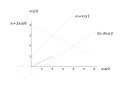
\includegraphics[width=\linewidth,keepaspectratio]{simplex_example}
	\end{center}
\end{minipage}

\begin{enumerate}[label=\arabic*.]
	\item $v = (2,3) \quad A = \begin{pmatrix}
	-1 & 1\\
	1 & 2\\
	2 & -3\\
	-1 & 0\\
	0 & -1
	\end{pmatrix} \quad b = \begin{pmatrix}
	1\\
	8\\
	2\\
	0\\
	0
	\end{pmatrix} \quad c = \begin{pmatrix}2\\1\end{pmatrix}$
	\begin{enumerate}[label=\arabic*)]
		\item $B = (1,2)$
		\item $A_B = \begin{pmatrix}
		-1 & 1\\
		1 & 2
		\end{pmatrix} \quad b_B = \begin{pmatrix}
		1\\
		8
		\end{pmatrix}$
		\item ${A_B}^{-1} = \frac{1}{-1\cdot2 - 1\cdot 1} \begin{pmatrix}
			2 & -1\\
			-1 & -1
		\end{pmatrix} = -\frac{1}{3} \begin{pmatrix}
		2 & -1\\
		-1 & -1
		\end{pmatrix} = \bordermatrix{~&-d&\cr
		~&-\frac{2}{3} & \frac{1}{3}\cr
		~&\frac{1}{3} & \frac{1}{3}\cr} = \bar{A}$
		\item $u = c^T \bar{A} = (2,1)\cdot \begin{pmatrix}
		-\frac{2}{3} & \frac{1}{3}\\
		\frac{1}{3} & \frac{1}{3}
		\end{pmatrix} = (-1,1) \ngeq \vec{0}$
		\item $Av = \begin{pmatrix}
		1\\
		8\\
		-5\\
		-2\\
		-3
		\end{pmatrix}\quad d = \begin{pmatrix}
		-\frac{2}{3}\\
		\frac{1}{3}
		\end{pmatrix} Ad = \begin{pmatrix}
		-1\\
		0\\
		\frac{7}{3}\\
		-\frac{2}{3}\\
		\frac{1}{3}
		\end{pmatrix} \quad \lambda = \begin{pmatrix}
		0\\
		0\\
		3\\
		-3\\
		9
		\end{pmatrix} \rightarrow \lambda^* = 3$
		\item $v' = v + \lambda^*\cdot d = \begin{pmatrix}2\\3\end{pmatrix} + 3\cdot \begin{pmatrix}-\frac{2}{3}\\\frac{1}{3}\end{pmatrix} = \begin{pmatrix}4\\2\end{pmatrix}$
	\end{enumerate}
	\item $v=(4,2)$
	\begin{enumerate}[label=\arabic*)]
		\item $B=(2,3)$
		\item $A_B = \begin{pmatrix}
		1 & 2\\
		2 & -3
		\end{pmatrix} \quad b_B = \begin{pmatrix}
		8\\
		2
		\end{pmatrix}$
		\item ${A_B}^{-1} = \frac{1}{1\cdot-3 - 2\cdot 2} \begin{pmatrix}
		-3 & -2\\
		-2 & 1
		\end{pmatrix} = \begin{pmatrix}
		\frac{3}{7} & \frac{2}{7}\\
		\frac{2}{7} & -\frac{1}{7}
		\end{pmatrix}$
		\item $u = (2,1)\begin{pmatrix}
		\frac{3}{7} & \frac{2}{7}\\
		\frac{2}{7} & -\frac{1}{7}
		\end{pmatrix} = (\frac{8}{7},\frac{3}{7}) \geq \vec{0}\quad\text{Vertex v is optimal}$
	\end{enumerate}
\end{enumerate}





\end{document}
